%\documentclass{beamer}
\documentclass[10pt]{beamer}

\usepackage{amsmath,amssymb,enumerate,calc,color,ifthen,capt-of,booktabs,graphicx,listings,algorithm2e,palatino,amsbsy,subfigure}

\usepackage{tikz}

\usefonttheme{serif}
 
\definecolor{light-gray}{gray}{0.95}
\lstset{basicstyle=\fontsize{7}{8}\selectfont\ttfamily,
        numbers=left,
        numberstyle=\fontsize{5}{6}\selectfont\ttfamily,
        numbersep=5pt,                  
        %backgroundcolor=\color{light-gray},
        frame=single, 
        %rulesepcolor=\color{red},
        keywordstyle=\color[rgb]{0,0,1},
        commentstyle=\color[rgb]{0.133,0.545,0.133},
        stringstyle=\color[rgb]{0.627,0.126,0.941},
        captionpos=b,
        title=\lstname,
        showstringspaces=false
       }


%---TITLE AND AUTHOR INFORMATION
\title % (optional, use only with long paper titles)
[C++ and Fortran]{Introduction to High-Performance and Parallel Computing}
\author[Roberts]{Prof.~Jeremy Roberts}
% \institute[22.213] % (optional, but mostly needed)
%  {}
% - Keep it simple, no one is interested in your street address.
\date
%[CFP 2003] % (optional, should be abbreviation of conference name)
{Fall 2017}


\begin{document}

% TITLE PAGE
\begin{frame}[plain]
  \titlepage
\end{frame}

% TABLE OF CONTENTS
\begin{frame}{Outline}
  \tableofcontents
  % You might wish to add the option [pausesections]
\end{frame}

%==============================================================================%

\section{Overview of Modern Computer Architectures}

%------------------------------------------------------------------------------%
\begin{frame}{Stored-Program Computer}

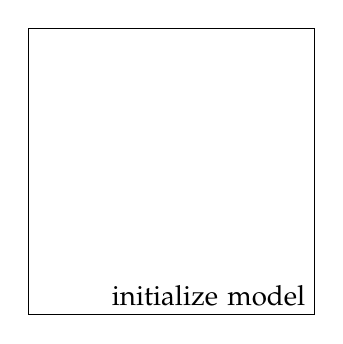
\begin{tikzpicture}
    \node [rectangle, draw, text width = 3.4cm, text height = 3.4cm, align = right] (init) {initialize model};
\end{tikzpicture}



\end{frame}


\section{Elements of Single-Core Optimization}


\section{Beyond Single-Core: Parallel Computing}


%------------------------------------------------------------------------------%
\begin{frame}{Flynn's Taxonomy}



\end{frame}



\end{document}
